\documentclass{article}
 
\usepackage[margin=1in]{geometry} 
\usepackage{amsmath,amsthm,amssymb,scrextend}
\usepackage{blindtext}
\usepackage{centernot}
\usepackage{enumerate}
\usepackage{enumitem}
\usepackage{fancyhdr}
\pagestyle{fancy}
\usepackage{babel}
\usepackage{pgfplots}
\usepackage{tikz}
\usepackage{wrapfig}

\pgfplotsset{compat=1.17}
 
\newcommand{\I}{\mathbb{I}}
\newcommand{\N}{\mathbb{N}}
\newcommand{\R}{\mathbb{R}}
\newcommand{\Q}{\mathbb{Q}}
\newcommand{\Z}{\mathbb{Z}}

\renewcommand{\qed}{\hfill$\blacksquare$}

\let\newproof\proof
\renewenvironment{proof}{\begin{addmargin}[1em]{0em}\begin{newproof}}{\end{newproof}\end{addmargin}\qed}

\newenvironment{corollary}[2][Corollary]{\begin{trivlist}
\item[\hskip \labelsep {\bfseries #1}\hskip \labelsep {\bfseries #2.}]}{\end{trivlist}}

\newenvironment{exercise}[2][Exercise]{\begin{trivlist}
\item[\hskip \labelsep {\bfseries #1}\hskip \labelsep {\bfseries #2.}]}{\end{trivlist}}

\newenvironment{lemma}[2][Lemma]{\begin{trivlist}
\item[\hskip \labelsep {\bfseries #1}\hskip \labelsep {\bfseries #2.}]}{\end{trivlist}}

\newenvironment{problem}[2][Problem]{\begin{trivlist}
\item[\hskip \labelsep {\bfseries #1}\hskip \labelsep {\bfseries #2.}]}{\end{trivlist}}

\newenvironment{proposition}[2][Proposition]{\begin{trivlist}
\item[\hskip \labelsep {\bfseries #1}\hskip \labelsep {\bfseries #2.}]}{\end{trivlist}}

\newenvironment{reflection}[2][Reflection]{\begin{trivlist}
\item[\hskip \labelsep {\bfseries #1}\hskip \labelsep {\bfseries #2.}]}{\end{trivlist}}

\newenvironment{theorem}[2][Theorem]{\begin{trivlist}
\item[\hskip \labelsep {\bfseries #1}\hskip \labelsep {\bfseries #2.}]}{\end{trivlist}}
 
\begin{document}

\lhead{Gabriel Hearot}
\rhead{\today}

\begin{problem}{1}
\blindtext
\end{problem}

\begin{wrapfigure}{l}{0.45\textwidth}
	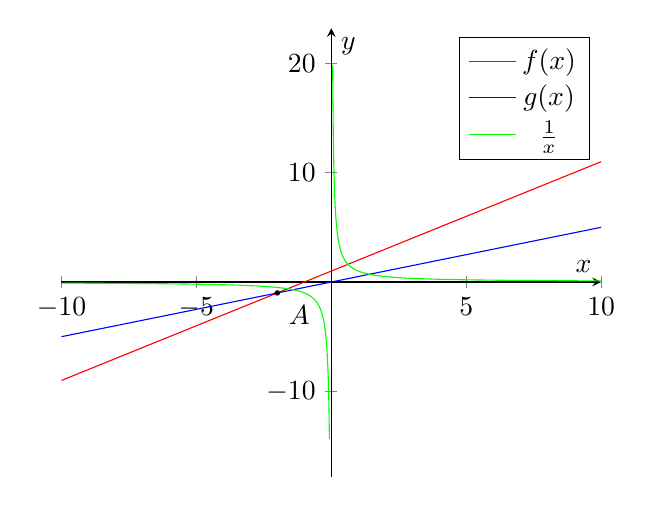
\begin{tikzpicture}
		\begin{axis}[
				axis lines = middle,
				no markers,
				xlabel = $x$,
				ylabel = $y$,
				enlarge y limits = true,
				enlarge x limits = false,
				restrict y to domain = -20:20,
			]
			\addplot [
				domain=-10:10, 
				samples=100, 
				color=red,
			]
			{\x+1};
			\addlegendentry{$f(x)$}
						
			\addplot [
				domain=-10:10, 
				samples=100, 
				color=blue,
			]
			{\x/2};
			\addlegendentry{$g(x)$}
						
			\addplot [
				smooth,
				domain=-10:10,
				samples=1000, 
				color=green,
			]
			{1/\x};
			\addlegendentry{$\frac{1}{x}$}
						
			\node[label={300:{$A$}},circle,fill,inner sep=0.7pt] at (axis cs:-2,-1) {};
		\end{axis}
	\end{tikzpicture}
		
	\caption{Lorem ipsum dolor sit amet.}
\end{wrapfigure}

\blindtext[2]

\vskip 0.2in

\begin{lemma}{1}
	\blindtext
\end{lemma}

\begin{wrapfigure}{l}{0.25\textwidth}
	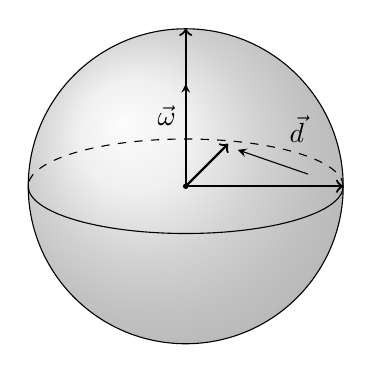
\begin{tikzpicture}[
			axis/.style={->,thick},
			vector/.style={-stealth},
		]
		\shade[ball color = gray!40, opacity = 0.4] (0,0) circle (2cm);
		\draw (0,0) circle (2cm);
		\draw (-2,0) arc (180:360:2 and 0.6);
		\draw[dashed] (2,0) arc (0:180:2 and 0.6);
		\fill[fill=black] (0,0) circle (1pt);
		\draw[axis] (0,0) -- (2,0,0);
		\draw[axis] (0,0) -- (0,0,-1.4);
		\draw[axis] (0,0) -- (0,2,0);
		  
		\draw[vector] (1.4,0,-0.4) -- node[label={55:$\vec{d}$}]{} (0.2,0,-1.2);
		\draw[vector] (0,0) -- node[anchor=south east]{$\vec{\omega}$} (0,1.3,0);
	\end{tikzpicture}
	
	\caption{Lorem ipsum dolor sit amet.}
\end{wrapfigure}

\blindmathpaper
\end{document}